\documentclass[11pt]{article}

\usepackage[margin=1in]{geometry}
\usepackage{amsmath,amssymb,amsthm,mathtools}
\usepackage{bm}
\usepackage{booktabs}
\usepackage{enumitem}
\usepackage{graphicx}
\usepackage{microtype}
\usepackage{tikz}
\usetikzlibrary{arrows.meta,positioning}
\usepackage[hidelinks]{hyperref}
\usepackage[nameinlink,noabbrev]{cleveref}
\usepackage[numbers,sort&compress]{natbib}
\usepackage{xcolor}

\newtheorem{theorem}{Theorem}[section]
\newtheorem{lemma}[theorem]{Lemma}
\newtheorem{proposition}[theorem]{Proposition}
\newtheorem{corollary}[theorem]{Corollary}
\theoremstyle{definition}
\newtheorem{definition}[theorem]{Definition}
\newtheorem{remark}[theorem]{Remark}

\newcommand{\Herm}{\operatorname{Herm}}
\newcommand{\Tr}{\operatorname{Tr}}
\newcommand{\rank}{\operatorname{rank}}
\newcommand{\conv}{\operatorname{conv}}
\newcommand{\supp}{\operatorname{supp}}
\newcommand{\id}{\mathbb I}
\newcommand{\R}{\mathbb R}
\newcommand{\C}{\mathbb C}
\newcommand{\Qset}{\mathsf Q}
\newcommand{\Qbar}{\overline{\mathsf Q}}
\newcommand{\POVM}{\mathrm{POVM}}
\newcommand{\PVM}{\mathrm{PVM}}
\newcommand{\Bell}{\mathcal B}
\newcommand{\cP}{\mathcal P}
\newcommand{\cR}{\mathcal R}
\newcommand{\cD}{\mathcal D}
\newcommand{\eps}{\varepsilon}

\title{\bfseries Minimum Input Complexity for Separating Qubit POVMs\\
from Projective Measurements}
\author{Alec Kriebel\\
\small Independent Researcher\\
\small \texttt{me@aleckriebel.com}\\
\small \url{https://aleckriebel.com/}}
\date{July 2026}

\begin{document}
\maketitle

\begin{abstract}
Earlier work showed that generalized qubit measurements can outperform
projective qubit measurements when one party has three Bell inputs and the
other has two. We prove the matching lower bound: two inputs per party never
suffice. For every choice of
finite, input-dependent output alphabets, every bipartite behavior generated
by qubit positive-operator-valued measurements belongs to the
shared-randomness convex hull of behaviors generated by qubit
projection-valued measurements. The statement permits arbitrary two-qubit
mixed states, zero projectors, deterministic relabeling, and stochastic
postprocessing, while forbidding dimension-increasing dilation. We also give
an explicit rational Bell functional with three inputs for one party and two
for the other whose value under an exact qubit POVM strategy strictly exceeds
a global analytic upper bound for every qubit projective strategy. Thus
\(3\times2\) is the minimum input architecture, up to exchanging the parties.
The equality proof reduces every possible two-input separator to a binary-
ternary residual architecture, models that architecture by a Lorentz
incidence manifold, obtains strictly positive multipliers from finite POVM
duality, and eliminates all ranks of the metric differential by second-order
geometry or explicit projective simulation.
\end{abstract}

\section{Introduction}

A positive-operator-valued measurement (POVM) is more general than a
projection-valued measurement (PVM) on a fixed Hilbert space. Naimark dilation
represents a POVM projectively only after adding degrees of freedom, so it
does not preserve a fixed local dimension. Bell experiments therefore offer
an operational question: how many measurement inputs are needed before
generalized measurements on local qubits generate correlations unavailable
to projective qubit measurements? This belongs to the broader study of Bell
nonlocality and dimension-constrained quantum behavior
\cite{brunner2014,navascues2015}.

Earlier work established that nonprojective qubit measurements can be useful
in Bell scenarios with three inputs on one side and two on the other
\cite{vertesi2010,barra2012}, and related device-independent constructions
certify nonprojective qubit measurements with larger input architectures
\cite{gomez2016}. This does not settle the two-input behavior-set question.
It also differs from operator-level projective simulability of individual
POVMs \cite{oszmaniec2017,guerini2017}: a Bell behavior may admit a projective
realization using a different state even when the original local POVM is not
itself a mixture of PVMs.

Strong reductions are known when every measurement is dichotomic
\cite{masanes2005,toner2006}; genuine ternary effects are precisely what those
arguments do not address. They also make exhaustive PVM conventions
essential. A published ternary-measurement claim was later corrected after a
qubit PVM with a zero effect was found to attain the same value
\cite{schwarz2016,schwarz2018corrigendum}. We therefore retain zero
projectors, deterministic inputs, every support pattern, and stochastic
postprocessing throughout.

\subsection*{Contributions}

We work throughout with local Hilbert-space dimension at most two and with
shared-randomness convexification. Our results are:

\begin{enumerate}[leftmargin=*,itemsep=3pt]
\item An explicit rational \(3\times2\) Bell functional has an exact
  algebraic qubit-POVM strategy above a global analytic upper bound for all
  qubit-PVM strategies (\cref{thm:separation}).
\item If one party has binary outcomes on both of its two inputs, every qubit
  POVM behavior is a common convex mixture of complete qubit-PVM behaviors
  (\cref{thm:binary-party}).
\item Any remaining strict two-input separator reduces to a pure entangled
  strategy with one binary PVM and one ternary rank-one POVM per party
  (\cref{thm:residual-reduction}).
\item The residual architecture cannot strictly exceed the PVM support
  function (\cref{thm:two-input-equality}). The proof treats every smooth and
  singular rank of an exact Lorentz incidence model.
\item Consequently \(3\times2\) is the minimum input architecture, up to
  exchanging the parties (\cref{cor:minimality}).
\end{enumerate}

\begin{figure}[t]
\centering
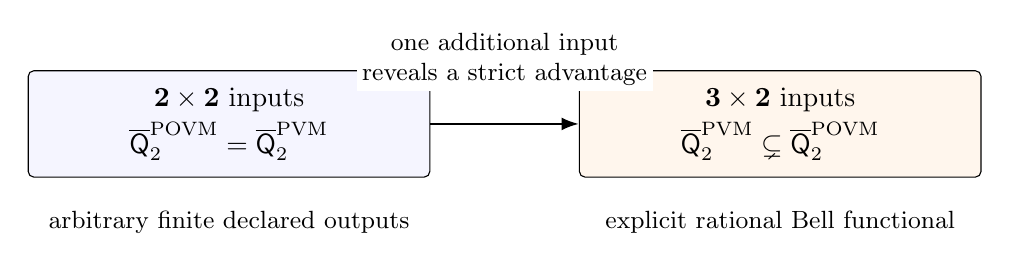
\begin{tikzpicture}[
  box/.style={draw,rounded corners=2pt,minimum width=5.1cm,
    minimum height=1.35cm,align=center,fill=blue!4},
  arr/.style={-{Latex[length=2.2mm]},thick},
  note/.style={align=center,font=\small}
]
\node[box] (two) at (0,0) {
  \(\mathbf{2\times2}\) inputs\\[1mm]
  \(\overline{\mathsf Q}^{\rm POVM}_2
    =\overline{\mathsf Q}^{\rm PVM}_2\)
};
\node[box,fill=orange!7] (three) at (7,0) {
  \(\mathbf{3\times2}\) inputs\\[1mm]
  \(\overline{\mathsf Q}^{\rm PVM}_2
    \subsetneq\overline{\mathsf Q}^{\rm POVM}_2\)
};
\draw[arr] (two) -- node[above=4mm,note,fill=white,inner sep=2pt]
  {one additional input\\reveals a strict advantage} (three);
\node[note] at (0,-1.25) {arbitrary finite declared outputs};
\node[note] at (7,-1.25) {explicit rational Bell functional};
\end{tikzpicture}

\caption{The minimum input threshold at fixed local dimension two. Equality
means equality after shared-randomness convexification for each fixed finite
declared-output architecture.}
\label{fig:threshold}
\end{figure}

The equality is not an operator identity between POVMs and PVMs, nor does it
assert simulation on the same state. It is an equality of convex behavior
sets. The distinction is central.

\subsection*{Proof roadmap}

The exact separation combines a CHSH locking term with a three-state
discrimination task. For the equality theorem, convex separation first turns
any counterexample into a global Bell maximizer. A Lorentz-cone circuit
argument handles every case in which one party is binary. A common-span
filtering perturbation and extremal-POVM dimension bound reduce all other
counterexamples to one binary and one ternary measurement per party.

In the residual architecture, the five local effects form a unique
binary-versus-ternary circuit. Lorentz coordinates describe the complete
strategy by a \(4\times4\) probability block \(P\) and a four-parameter
metric \(g\), subject to five quadratic null equations. Finite POVM duality
makes every determinant multiplier strictly positive at a hypothetical strict
separator. The constrained second variation then has ambient inertia
\((4,12)\). If the metric differential has rank at least two, dimension alone
forces an uphill direction. Rank one contradicts positivity through an exact
projective-fiber theorem, while rank zero has an explicit deterministic
decomposition.

\section{Model and convexified behavior sets}
\label{sec:model}

Let \(X=Y=\{0,1\}\) unless stated otherwise. Each input has a finite declared
output alphabet \(A_x\) or \(B_y\), which may depend on the input.

\begin{definition}[Fixed-qubit behavior]
A single fixed-qubit POVM strategy consists of Hilbert spaces
\(\mathcal H_A,\mathcal H_B\) of dimensions at most two, a density operator
\(\rho\) on \(\mathcal H_A\otimes\mathcal H_B\), and effects
\[
 M^x_a\ge0,\quad \sum_{a\in A_x}M^x_a=\id_A,\qquad
 N^y_b\ge0,\quad \sum_{b\in B_y}N^y_b=\id_B.
\]
It produces
\[
 p(a,b|x,y)=\Tr\!\left[\rho(M^x_a\otimes N^y_b)\right].
\]
The resulting set is denoted
\(\Qset^{\POVM}_2(\mathbf A,\mathbf B)\).
\end{definition}

A PVM strategy requires all effects in each measurement to be mutually
orthogonal projections. Zero projections are permitted. Therefore a
qubit PVM with arbitrarily many declared labels has at most two nonzero
effects. No ancillary system or Naimark dilation may increase a local
dimension above two.

We denote the shared-randomness hulls by
\[
\Qbar^{\POVM}_2(\mathbf A,\mathbf B)
 :=\conv\Qset^{\POVM}_2(\mathbf A,\mathbf B),\qquad
\Qbar^{\PVM}_2(\mathbf A,\mathbf B)
 :=\conv\Qset^{\PVM}_2(\mathbf A,\mathbf B).
\]
Local stochastic postprocessing is included on the PVM side.

\begin{lemma}[Convexification and postprocessing]
\label{lem:convexification}
For a linear Bell functional, shared randomness and stochastic
postprocessing do not increase the optimum beyond one deterministic
projective component.
\end{lemma}

\begin{proof}
Linearity gives
\[
\mathcal F\!\left(\sum_\lambda q_\lambda p_\lambda\right)
=\sum_\lambda q_\lambda\mathcal F(p_\lambda)
\le\max_\lambda\mathcal F(p_\lambda).
\]
A finite stochastic map is a convex combination of deterministic maps.
Absorb all deterministic choices into the shared variable. A deterministic
map merges mutually orthogonal projectors assigned to the same displayed
label and inserts zero projectors for unused labels, hence remains a declared-
output PVM.
\end{proof}

For fixed finite alphabets, all strategy spaces above are compact. Indeed,
density matrices and tuples of effects form closed bounded sets in
finite-dimensional matrix spaces, and the Born map is continuous. The convex
hull of a compact subset of a finite-dimensional affine space is compact:
affine dependence reduces every convex combination to at most \(m+1\) points
in affine dimension \(m\).

\begin{lemma}[Nearest-point separation]
\label{lem:nearest}
Let \(\cP\) be a compact convex subset of a finite-dimensional Euclidean
space. If \(q\notin\cP\) and \(p_0\) minimizes \(\|q-p\|\) over \(p\in\cP\),
then \(c=q-p_0\) satisfies
\[
c\cdot q>\sup_{p\in\cP}c\cdot p.
\]
\end{lemma}

\begin{proof}
For \(p\in\cP\), differentiate
\(\|q-p_0-t(p-p_0)\|^2\) at \(t=0^+\). Minimality gives
\((q-p_0)\cdot(p-p_0)\le0\), and strictness follows from \(q\ne p_0\).
\end{proof}

\begin{remark}[Notation for arbitrary outputs]
The shorthand
\(\Qbar^{\POVM}_2(2,2)=\Qbar^{\PVM}_2(2,2)\) means an equality schema:
the equality holds separately for every choice of finite
\((A_0,A_1;B_0,B_1)\). It is not an identification of behavior vectors
living in different ambient spaces.
\end{remark}

\section[An exact rational 3-by-2 separation]
{An exact rational \(3\times2\) separation}
\label{sec:separation}

For this section take Alice inputs \(x=0,1,2\), Bob inputs \(y=0,1\), Alice
labels \(a=0,1,2\), and Bob labels \(b=0,1\). Define signs
\[
\alpha_0=\alpha_2=1,\quad\alpha_1=-1,\qquad
\beta_0=1,\quad\beta_1=-1
\]
and correlators
\[
E_{xy}=\sum_{a,b}\alpha_a\beta_b\,p(a,b|x,y).
\]
Set
\begin{equation}
\label{eq:bell-functional}
\begin{aligned}
\Bell(p)={}&10(E_{00}+E_{01}+E_{10}-E_{11})\\
&+\frac35p(0,0|2,0)+\frac35p(1,1|2,0)
 +\frac45p(2,0|2,1).
\end{aligned}
\end{equation}
For this declared-output architecture, write
\[
\beta_{\POVM}(\Bell)
:=\sup_{p\in\Qbar^{\POVM}_2}\Bell(p),\qquad
\beta_{\PVM}(\Bell)
:=\sup_{p\in\Qbar^{\PVM}_2}\Bell(p).
\]

\begin{theorem}[Exact fixed-qubit separation]
\label{thm:separation}
For the rational functional \eqref{eq:bell-functional},
\[
\beta_{\POVM}(\Bell)\ge
L_1:=\frac{16+8\sqrt{7813}}{25}
>
U:=20\sqrt2+\frac35+\frac{4+3\sqrt2}{250}
\ge\beta_{\PVM}(\Bell).
\]
The certified gap is
\[
L_1-U=\frac{6+80\sqrt{7813}-5003\sqrt2}{250}>0.
\]
These are an attained POVM lower bound and a global PVM upper bound; neither
is asserted to be the corresponding exact optimum.
\end{theorem}

\subsection{The simple exact strategy}

Let \(X,Z\) be Pauli matrices and
\[
|\Phi^+\rangle=(|00\rangle+|11\rangle)/\sqrt2.
\]
Bob uses \(B_0=Z\), \(B_1=X\). Alice uses
\[
A_0=(Z+X)/\sqrt2,\qquad A_1=(Z-X)/\sqrt2
\]
for her first two binary measurements, with a zero third label. Her final
measurement is
\[
\begin{aligned}
M_0&=(17\id-8X+15Z)/50,\\
M_1&=(17\id-8X-15Z)/50,\\
M_2&=(16\id+16X)/50.
\end{aligned}
\]
The rank-one factorizations
\[
M_0=\frac1{25}\binom4{-1}(4,-1),\quad
M_1=\frac1{25}\binom1{-4}(1,-4),\quad
M_2=\frac8{25}\binom11(1,1)
\]
prove positivity and normalization. Their nonzero eigenvalues are
\(17/25,17/25,16/25\), so the measurement is not a PVM.

The identity
\[
\langle\Phi^+|R\otimes S|\Phi^+\rangle
=\frac12\Tr(R^TS)
\]
gives CHSH value \(2\sqrt2\) and
\[
p(0,0|2,0)=p(1,1|2,0)=p(2,0|2,1)=\frac8{25}.
\]
Thus the simpler value
\[
L_0=20\sqrt2+\frac{16}{25}
\]
already exceeds \(U\), since
\[
L_0-U=\frac{3(2-\sqrt2)}{250}>0.
\]

At the ideal point the auxiliary term is a state-discrimination problem with
\[
W_0=\frac3{20}(\id+Z),\quad
W_1=\frac3{20}(\id-Z),\quad
W_2=\frac15(\id+X).
\]
The dual operator
\[
\Gamma=\frac8{25}\id+\frac2{25}X
\]
satisfies \(\Gamma\ge W_i\) and
\((\Gamma-W_i)M_i=0\), so the POVM value is \(16/25\).
Every one- or two-label qubit PVM support scores at most \(3/5\). The ideal
discrimination advantage is therefore \(1/25\).

\subsection{Global projective bound}

Write \(\Bell=10S+T\). For a PVM strategy, the displayed CHSH observables are
Hermitian unitaries, including possible values \(\pm\id\). If one is
degenerate, the CHSH identity
\[
C_{\rm CHSH}^2
=4\id-[A_0,A_1]\otimes[B_0,B_1]
\]
gives \(S\le2\), while \(T\le7/5\), which is below \(U\).

Otherwise optimize the state to a pure state and put it in Schmidt form
\[
|\psi_\eta\rangle=
\sqrt{\frac{1+\eta}{2}}|00\rangle+
\sqrt{\frac{1-\eta}{2}}|11\rangle,\qquad0\le\eta\le1.
\]
Its correlation matrix is
\[
R=\operatorname{diag}(\sqrt{1-\eta^2},-\sqrt{1-\eta^2},1).
\]
If \(u=|\bm b_0\cdot\bm b_1|\) and
\(\delta=2\sqrt2-S\), optimizing Alice's directions and applying
Cauchy--Schwarz gives
\begin{equation}
\label{eq:deficit-bounds}
S\le2\sqrt2-\frac{\eta^2}{\sqrt2},\qquad
S\le2\sqrt2-\frac{u^2}{2\sqrt2},
\end{equation}
hence
\[
\eta\le2^{1/4}\sqrt\delta,\qquad
u\le2^{3/4}\sqrt\delta.
\]

A ternary qubit PVM has one of the six labeled rank patterns obtained by
permuting \((2,0,0)\) or \((1,1,0)\). For every singleton support and the
pair \(\{0,1\}\), \(T\le3/5+2(\eta+u)/5\). A pair involving label \(2\)
reduces to binary discrimination between
\[
\Pi(\bm v):=\frac12(\id+\bm v\cdot\bm\sigma),\qquad
A=\frac35D \Pi(\bm n)D,\qquad
B=\frac45D \Pi(\bm m)D,
\quad
D=\operatorname{diag}\!\left(
\sqrt{\frac{1+\eta}{2}},\sqrt{\frac{1-\eta}{2}}\right).
\]
With \(x=n_z\), \(y=m_z\), and \(r=\bm n\cdot\bm m\),
\[
20F_\eta
=7+\eta(3x+4y)
+\sqrt{[-1+\eta(3x-4y)]^2+24(1-\eta^2)(1-r)}.
\]
The exact comparison
\[
F_\eta\le F_0(r)+\frac{2\eta}{5}
\le\frac35+\frac25(\eta+u)
\]
is proved by the manifestly nonnegative polynomial certificate in
\cref{app:separation-algebra}. Consequently
\[
T\le\frac35+\frac25(\eta+u)
\le\frac35+C\sqrt\delta,
\quad
C=\frac25(2^{1/4}+2^{3/4}),
\]
where \(C^2=(16+12\sqrt2)/25\). Completing the square,
\[
\Bell\le20\sqrt2+\frac35+C\sqrt\delta-10\delta
\le20\sqrt2+\frac35+\frac{C^2}{40}=U.
\]
This covers every state, support pattern, direction, relabeling, and
degeneracy. \Cref{lem:convexification} covers shared randomness and
postprocessing. The stronger algebraic strategy attaining \(L_1\) and exact
gap comparison are given in \cref{app:strengthened}.

\section{Two-input reductions}
\label{sec:reductions}

\subsection{One binary party}

\begin{theorem}[One-binary-party simulation]
\label{thm:binary-party}
Suppose one party in a two-input bipartite qubit scenario has binary declared
outputs on both inputs. The other party may have arbitrary finite outputs.
Then every qubit-POVM behavior belongs to the convex hull of fixed-qubit PVM
behaviors. The statement is symmetric under exchanging the parties.
\end{theorem}

\begin{proof}
Decompose each binary qubit POVM into PVMs. If \(E\) has eigenvalues
\(0\le\mu\le\lambda\le1\) and \(P\) is the spectral projector for \(\lambda\),
then
\[
\{E,\id-E\}=(\lambda-\mu)\{P,\id-P\}
+\mu\{\id,0\}+(1-\lambda)\{0,\id\}.
\]
Taking the product of the decompositions for both inputs reduces, in each
shared-random component, Bob to fixed binary PVMs with observables \(B_0,B_1\).

For Alice outcome \(a|x\), let \(\sigma_{a|x}\) be Bob's subnormalized steered
state and define
\[
\Phi_B(\sigma)=
\bigl(\Tr\sigma,\Tr(\sigma B_0),\Tr(\sigma B_1)\bigr)\in\R^3.
\]
These data determine all joint probabilities:
\[
p(a,b|x,y)=\frac12\left[
(\Phi_B\sigma_{a|x})_0+(-1)^b(\Phi_B\sigma_{a|x})_{y+1}
\right].
\]
No-signaling gives equality of the sums of the two compressed ensembles.

If \(\id,B_0,B_1\) are linearly independent, the image of the positive
qubit cone is a three-dimensional Lorentz cone: the cone over the elliptical
projection of the Bloch ball onto the span of the two Bloch axes. Parallel,
antiparallel, or scalar observables give a two-dimensional simplicial cone or
a local deterministic degeneration; these cases are included in
\cref{app:binary-degeneracies}.

Decompose every compressed positive vector into extreme rays, retaining its
original output label. Repeatedly extract support-minimal positive
subrelations. In real dimension at most three, such a circuit has at most four
distinct signed rays. A one-versus-many relation would express an extreme ray
as a positive sum of different cone rays and is impossible. Collinear
one-versus-one relations are zero-padded binary components. Every nontrivial
circuit is therefore
\[
r_0+r_1=s_0+s_1.
\]

Every extreme compressed ray has a unique positive rank-one lift inside
\(\operatorname{span}_{\R}\{\id,B_0,B_1\}\). Thus the circuit lifts to
\[
R_0+R_1=S_0+S_1=\Omega
\]
between rank-one positive operators. If \(\Omega\) is invertible, the two
rank-one decompositions become two orthonormal bases after applying
\(\Omega^{-1/2}\). The canonical purification
\[
|\Psi_\Omega\rangle=
(\id\otimes\sqrt{\Omega/\Tr\Omega})(|00\rangle+|11\rangle)
\]
therefore realizes both ensembles by two Alice PVMs. Rank-one \(\Omega\),
zero terms, and repeated rays require a little bookkeeping. If
\(\Omega=|\omega\rangle\langle\omega|\) has rank one, every nonzero summand
is collinear with \(\Omega\), so
\[
R_i=\rho_i\Omega,\quad S_i=\sigma_i\Omega,\qquad
\rho_0+\rho_1=\sigma_0+\sigma_1=1.
\]
A product purification with Bob state proportional to \(\Omega\), together
with independently chosen Alice PVM bases, realizes the two arbitrary binary
weight vectors \((\rho_0,\rho_1)\) and \((\sigma_0,\sigma_1)\). Zero terms
receive zero projectors. Collinear terms are combined only within their
retained output labels; if the same geometric ray occurs under different
labels, classical splitting restores those labels branchwise. Thus no
outcome probability is lost when repeated rays are removed.

Give this circuit strategy shared weight \(\Tr\Omega\). Circuit elimination
preserves total trace, so the weights sum to one. The retained output labels
and fixed Bob PVMs reconstruct every original compressed vector and hence
every joint probability. This is one common decomposition of the complete
behavior, not a separate decomposition for each input.
\end{proof}

\subsection{Extreme residual architecture}

\begin{lemma}[Common-span filtering]
\label{lem:common-span}
Let Alice's two POVMs have a common Hermitian combination
\[
H=\sum_a s_{a|0}M_{a|0}=\sum_a s_{a|1}M_{a|1}.
\]
For sufficiently small \(\eps>0\), define
\[
S_\pm=\id\pm\eps H,\quad
r^\pm_{a|x}=1\pm\eps s_{a|x},
\]
\[
M^\pm_{a|x}
=r^\pm_{a|x}S_\pm^{-1/2}M_{a|x}S_\pm^{-1/2}.
\]
With
\[
q_\pm=\Tr[(S_\pm\otimes\id)\rho],\qquad
\rho_\pm=
\frac{(S_\pm^{1/2}\otimes\id)\rho(S_\pm^{1/2}\otimes\id)}
{q_\pm},
\]
the original complete behavior satisfies
\[
p=\frac{q_+}{2}p_++\frac{q_-}{2}p_-.
\]
\end{lemma}

\begin{proof}
The effects normalize because
\(\sum_a r^\pm_{a|x}M_{a|x}=S_\pm\), and \(q_++q_-=2\).
Direct cyclicity of trace gives
\[
q_\pm p_\pm(a,b|x,y)=r^\pm_{a|x}p(a,b|x,y).
\]
Averaging the signs proves the identity for all inputs and outputs.
\end{proof}

\begin{theorem}[Residual-architecture reduction]
\label{thm:residual-reduction}
If a Bell functional with two inputs per party has a strict qubit-POVM advantage over
\(\Qbar^{\PVM}_2\), a global maximizing component may be chosen with:
\begin{enumerate}[label=(\roman*),itemsep=2pt]
\item a pure full-Schmidt-rank two-qubit state;
\item one nondegenerate binary PVM on each party;
\item one extremal ternary rank-one POVM on each party;
\item local real measurement spans intersecting only in \(\R\id\).
\end{enumerate}
In particular, four-outcome extremal POVMs are unnecessary.
\end{theorem}

\begin{proof}
Choose an extreme point of the exposed maximizing face. Compactness and
extremality let us select one unrandomized realization. Decompose its state
into pure states while holding the measurements fixed; every positive-weight
component must produce the same extreme behavior. A product state is local,
so select a pure entangled state, whose reduced states are full rank.

Likewise decompose each local POVM into extremal POVMs, one measurement at a
time. Extremality permits an extremal component that still realizes the same
behavior. Temporarily delete zero effects; they contribute no probabilities
and their declared output labels can be reinserted at the end. Full-rank
reduced states then make every remaining outcome marginal strictly positive.
For one party set
\[
V_x=\operatorname{span}_{\R}\{M_{a|x}\}\subset\Herm(2).
\]
If \(V_0\cap V_1\) contained a nonscalar \(H\), \cref{lem:common-span} would
split the behavior. Equality of both branch behaviors would imply, using
strictly positive outcome marginals,
\(r^\pm_{a|x}=q_\pm\) for every nonzero outcome, making all coefficients
equal and \(H\) scalar. Thus
\[
V_0\cap V_1=\R\id.
\]

Since \(\dim_{\R}\Herm(2)=4\), one of \(V_0,V_1\) has dimension at most two.
It is commuting and is a stochastic postprocessing of a binary spectral PVM.
Behavior extremality selects a deterministic postprocessing, so this input
may be taken as a PVM. Retain an extreme deterministic component realizing the
same behavior and apply \cref{lem:common-span} once more to that realization;
its two final measurement spans therefore still intersect only in
\(\R\id\). The PVM is nondegenerate, because a party with only one nontrivial
input produces a local behavior.

The other span has dimension at most three. Its nonzero effects are linearly
independent; otherwise \cref{lem:common-span} with \(H=0\) splits the extreme
behavior. For an extremal qubit POVM, support-preserving perturbations give
\[
\sum_a\rank(M_a)^2\le4.
\]
The standard extremality criterion \cite{dariano2005,haapasalo2012} is
reproved in \cref{app:extremal-povm} for completeness.
A genuine nonprojective measurement in a three-dimensional span therefore
has exactly three nonzero rank-one effects. If both spans on one party were
at most two, \cref{thm:binary-party} would make the full behavior
PVM-simulable. Apply the argument to both parties, then reinsert any deleted
zero-output labels.
\end{proof}

\section{Lorentz incidence model}
\label{sec:incidence}

Write every Hermitian \(2\times2\) matrix as
\[
X=x_0\id+x_1\sigma_x+x_2\sigma_y+x_3\sigma_z
\]
and set \(J=\operatorname{diag}(1,-1,-1,-1)\). Then
\[
\det X=x^TJx.
\]
Nonzero positive rank-one effects are precisely future-null vectors:
\(x_0>0\), \(x^TJx=0\).

In the residual architecture label one party's two binary effects by
\(E_1,E_2\) and ternary effects by \(E_3,E_4,E_5\). Set
\[
r_1=e_1,\ r_2=e_2,\ r_3=e_3,\ r_4=e_4,\quad
r_5=(1,1,-1,-1)^T,\quad u=(1,1,0,0)^T.
\]
Their unique coefficient circuit is
\[
r_1+r_2=r_3+r_4+r_5=u.
\]

\begin{figure}[t]
\centering
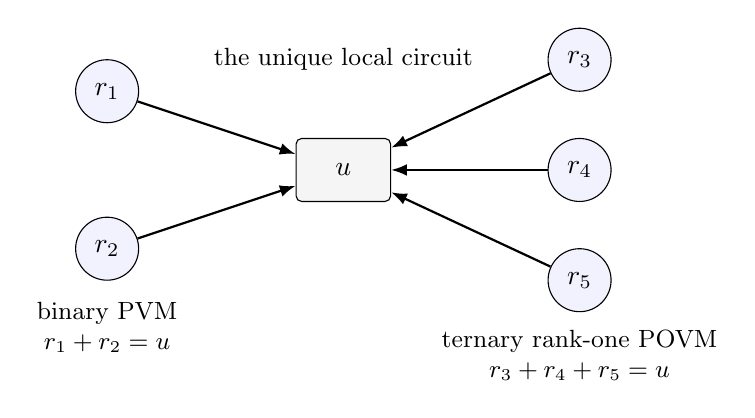
\begin{tikzpicture}[
  ray/.style={circle,draw,minimum size=8mm,inner sep=0pt,fill=blue!5},
  sum/.style={rectangle,draw,rounded corners=2pt,minimum width=12mm,
    minimum height=8mm,fill=gray!8},
  arr/.style={-{Latex[length=2mm]},thick}
]
\node[ray] (r1) at (-3,1.0) {\(r_1\)};
\node[ray] (r2) at (-3,-1.0) {\(r_2\)};
\node[sum] (u) at (0,0) {\(u\)};
\node[ray] (r3) at (3,1.4) {\(r_3\)};
\node[ray] (r4) at (3,0) {\(r_4\)};
\node[ray] (r5) at (3,-1.4) {\(r_5\)};
\draw[arr] (r1) -- (u);
\draw[arr] (r2) -- (u);
\draw[arr] (r3) -- (u);
\draw[arr] (r4) -- (u);
\draw[arr] (r5) -- (u);
\node[align=center,font=\small] at (-3,-2.0) {binary PVM\\\(r_1+r_2=u\)};
\node[align=center,font=\small] at (3,-2.35) {ternary rank-one POVM\\\(r_3+r_4+r_5=u\)};
\node[align=center,font=\small] at (0,1.4) {the unique local circuit};
\end{tikzpicture}


\caption{The local coefficient circuit after choosing four effects as an
operator basis. The physical effects are future-null rays in a Lorentz
metric.}
\label{fig:circuit}
\end{figure}

The first four physical effects form a real basis of \(\Herm(2)\). Let
\(\mathsf E\) contain their Lorentz vectors as columns and define
\(g=\mathsf E^TJ\mathsf E\). Nullness and normalization force
\begin{equation}
\label{eq:metric}
g=
\begin{pmatrix}
0&\tfrac12&a&b\\
\tfrac12&0&c&d\\
a&c&0&e\\
b&d&e&0
\end{pmatrix},
\qquad e=a+b+c+d-\tfrac12.
\end{equation}
On the genuine residual stratum all distinct-ray products are positive; in
particular \(a,b,c,d,e>0\) and
\[
a+b,c+d,a+c,b+d<\frac12.
\]

Choose the first four effects on both parties as bases and let \(P\) be their
\(4\times4\) joint-probability block. The complete table is
\[
p_{ij}=r_i^TPr_j,\qquad u^TPu=1.
\]
For a pure full-Schmidt-rank state
\(|\psi_C\rangle=\sum C_{mn}|mn\rangle\), steering is
\(\Theta_C(N)=CN^TC^\dagger\). Its Lorentz matrix \(L_C\) satisfies
\[
L_C^TJL_C=|\det C|^2J.
\]
If \(h\) is Bob's local metric, then
\[
P^Tg^{-1}P=4|\det C|^2h.
\]
Thus \(P\) is invertible. With \(Q=g^{-1}\), define
\begin{equation}
\label{eq:incidence}
F_j(P,g):=(Pr_j)^TQ(Pr_j)=0,\qquad j=1,\ldots,5.
\end{equation}

\section{Physical exactness and smoothness}
\label{sec:physical}

\begin{theorem}[Local physical completeness]
\label{thm:physical-completeness}
Near every genuine residual point, every nearby \((P,g)\) satisfying
\eqref{eq:metric}, the five incidence equations \eqref{eq:incidence},
normalization, Lorentz signature, and the strict time-orientation inequalities
is realized by a genuine residual two-qubit strategy. Every incidence tangent
therefore integrates to a two-sided physical curve.
\end{theorem}

\begin{proof}
Because \(g\) has signature \((1,3)\), \(u^Tgu=1\), and the restriction to
\(u^{\perp_g}\) is negative definite, Lorentz Gram--Schmidt gives a smoothly
varying \(\mathsf E\) with
\[
\mathsf E^TJ\mathsf E=g,\qquad
\mathsf E u=(1,0,0,0)^T.
\]
Each \(r_i\) is \(g\)-null and has positive product with \(u\); hence
\(\mathsf E r_i\) is future null and represents a positive rank-one Alice
effect. The circuit makes both measurements sum to the identity.

Put \(x_j=Pr_j\) and
\[
s_j=\frac12\mathsf E^{-T}x_j.
\]
The incidence equations give \(s_j^TJs_j=0\), while
\(2(s_j)_0=u^Tx_j\) is the strictly positive Bob marginal. Thus \(s_j\)
represents a future-null positive rank-one steered operator \(S_j\).
The circuit yields
\[
S_1+S_2=S_3+S_4+S_5=:\rho_A.
\]
Normalization gives \(\Tr\rho_A=1\), and full rank is open near the original
point. Let \(C=\rho_A^{1/2}\) and set
\[
N_j^T=C^{-1}S_jC^{-\dagger}.
\]
The \(N_j\) are positive rank-one effects and normalize on both inputs.
Moreover
\[
\Tr(E_iS_j)=r_i^TPr_j,
\]
so every reconstructed probability is physical and nonnegative.

The six constraints below have independent differentials, so the regular
level-set theorem supplies local coordinates and integrates every tangent.
Signature, time orientation, positive marginals, and full rank are open
conditions, giving a two-sided physical curve for sufficiently small
parameter values even when a joint probability is zero.
\end{proof}

\begin{proposition}[Smooth incidence manifold]
\label{prop:smooth}
Restricted to the open genuine residual stratum---in particular, where
\(g\) has Lorentz signature, all strict time-orientation inequalities hold,
and \(P\) is invertible---the normalized incidence space is a smooth real
\(14\)-dimensional manifold.
\end{proposition}

\begin{proof}
\[
\nabla_PF_j=2QPr_jr_j^T.
\]
If a linear combination vanishes, invertibility of \(QP\) gives
\[
\sum_j\mu_jr_jr_j^T
=\operatorname{diag}(\mu_1,\ldots,\mu_4)+\mu_5r_5r_5^T=0.
\]
Off-diagonal entries first give \(\mu_5=0\), then diagonal entries give all
other coefficients zero. Normalization is independent because the radial
variation \(\delta P=P\) annihilates every \(dF_j\) but changes \(u^TPu\).
There are \(16+4-5-1=14\) dimensions.
\end{proof}

\begin{remark}
The proposition is local to the open stratum used by the residual closure;
singular normalized incidence points outside that stratum are not asserted to
be smooth. The projected behavior image has dimension at most \(14\); no claim
of exact projected dimension is needed for the closure theorem.
\end{remark}

\section{Stationarity and strictly positive multipliers}
\label{sec:multipliers}

Every entry of the complete residual behavior is \(r_i^TPr_j\). Thus, after
collecting the original Bell coefficients into numbers
\(\gamma_{ij}\), its restriction to the incidence coordinates is the linear
objective
\[
L_{\mathsf C}(P):=\sum_{i,j}\gamma_{ij}r_i^TPr_j
=\Tr(\mathsf C^TP),\qquad
\mathsf C:=\sum_{i,j}\gamma_{ij}r_ir_j^T.
\]
At a stationary point, the six constraint gradients are linearly independent.
Thus there are unique multipliers
\(\alpha,\lambda_1,\ldots,\lambda_5\), with sign convention
\begin{equation}
\label{eq:lagrange}
\mathsf C-\alpha uu^T=-2QP\Lambda,\qquad
\Lambda=\sum_{j=1}^5\lambda_jr_jr_j^T.
\end{equation}
Stationarity in the four metric variables says
\(\lambda\in\ker\cD^T\), where \(\cD\) is defined in
\cref{sec:second-variation}.

\begin{lemma}[Finite POVM duality]
\label{lem:povm-duality}
For
\[
\max_{N_j\ge0,\ \sum_jN_j=\id}\sum_j\Tr(K_jN_j),
\]
there is a Hermitian \(\Gamma\) such that
\[
\Gamma\ge K_j,\qquad(\Gamma-K_j)N_j=0.
\]
\end{lemma}

\begin{proof}
Weak duality is immediate. Strong duality follows by separating the closed
finite-dimensional cone
\[
\left\{\left(\sum_jX_j,\sum_j\Tr(K_jX_j)-t\right):
X_j\ge0,\ t\ge0\right\}
\]
from \((\id,V+\eps)\), where \(V\) is the primal optimum, and taking
\(\eps\downarrow0\). Equality of primal and dual values gives
\[
\sum_j\Tr[(\Gamma-K_j)N_j]=0.
\]
Every summand is nonnegative, hence zero; for positive matrices,
\(\Tr(AB)=0\) implies \(AB=0\). Full details are included in
\cref{app:duality}.
\end{proof}

\begin{proposition}[Strict multiplier positivity]
\label{prop:positive-multipliers}
At a residual global Bell maximizer whose value is strictly above the PVM
support value,
\[
\lambda_j>0\quad(j=1,\ldots,5),\qquad\Lambda>0.
\]
\end{proposition}

\begin{proof}
For each Bob input \(y\), hold the state and all other measurements fixed and
collect the terms of \(L_{\mathsf C}\) depending on that input as
\[
\sum_{j\in B_y}\Tr(K_{j|y}N_{j|y}).
\]
Within one input abbreviate \(K_{j|y}\) and \(N_{j|y}\) by \(K_j,N_j\).
Apply \cref{lem:povm-duality} separately to Bob's binary and ternary inputs,
with distinct normalization operators \(\Gamma_y\). A nonzero rank-one
qubit effect satisfies
\[
\Gamma_y-K_j=s_j\operatorname{adj}(N_j),\qquad s_j\ge0,
\]
and \(\operatorname{adj}(N_j)N_j=0\).

Under full-rank steering,
\[
F_j=4|\det C|^2\det N_j.
\]
Pulling \eqref{eq:lagrange} back to variations of the effects on input \(y\)
gives
\[
K_j-\Gamma_y+
4|\det C|^2\lambda_j\operatorname{adj}(N_j)=0.
\]
The normalization operator here is the dual operator: if two candidates
satisfy complementary slackness, their difference annihilates the range of
every effect in that input, and those ranges span \(\C^2\) because the
effects sum to \(\id\). Therefore
\[
4|\det C|^2\lambda_j=s_j\ge0.
\]

If \(s_j=0\), then \(K_j=\Gamma_y\). Replacing that entire input by the
deterministic PVM \(N_j=\id\), \(N_k=0\) preserves the score. That party now
has only one nontrivial input. Every corresponding nonsignaling behavior is
local: use the output of the nontrivial input as a hidden variable and sample
the other party's potential outputs conditionally. Deterministic local
behaviors use only identity and zero projectors. A strict value above the PVM
support therefore forces every \(s_j\), and hence every \(\lambda_j\), to be
positive. Since \(r_1,\ldots,r_4\) form a basis, \(\Lambda>0\).
\end{proof}

\section{Exact second variation}
\label{sec:second-variation}

A tangent metric variation has the form
\[
H(A,B,C,D)=
\begin{pmatrix}
0&0&A&B\\
0&0&C&D\\
A&C&0&A+B+C+D\\
B&D&A+B+C+D&0
\end{pmatrix}.
\]
Define
\[
\Phi(y)=
\begin{pmatrix}
y_2(y_0+y_3)\\
y_3(y_0+y_2)\\
y_2(y_1+y_3)\\
y_3(y_1+y_2)
\end{pmatrix},
\quad y_j=QPr_j,
\]
and
\[
\cD:H\longmapsto(y_1^THy_1,\ldots,y_5^THy_5).
\]
Then
\[
\rank\cD=\dim\operatorname{span}\{\Phi(y_1),\ldots,\Phi(y_5)\}.
\]
Let \(K=\ker\cD^T\), \(k=\dim K=5-\rank\cD\). Metric stationarity says
\(\lambda\in K\).

For a tangent \((\delta P,H)\), set
\[
S=P^TQP,\qquad \delta P=PW+HQ P.
\]
The first-order equations are solvable for \(H\) exactly when
\[
\Tr(SW\Lambda_\mu)=0\quad(\mu\in K),
\qquad
\Lambda_\mu=\sum_j\mu_jr_jr_j^T.
\]
The compatible space
\[
\mathcal H_K=
\{W:\Tr(SW\Lambda_\mu)=0\ \forall\mu\in K\}
\]
has dimension \(16-k\).

\begin{proposition}[Weighted second form]
\label{prop:second-form}
\[
\sum_j\lambda_jD^2F_j=2q(W),\qquad
q(W)=\Tr(SW\Lambda W^T),
\]
and
\[
\operatorname{inertia}(q)=(4,12).
\]
Every positive-\(q\) compatible tangent can be adjusted to satisfy
normalization without changing \(q\).
\end{proposition}

\begin{proof}
Differentiating \(g^{-1}\) twice and completing the square after
\(\delta P=PW+HQ P\) gives
\[
D^2F_j=2(PWr_j)^TQ(PWr_j),
\]
and summing against \(\lambda_j\) yields the trace formula. The exact
expansion is recorded in \cref{app:square-completion} and independently
checked by the verifier.

The matrix \(S\) has signature \((1,3)\), while \(\Lambda>0\).
Invertible congruences therefore reduce \(q\) to
\[
q_0(Z)=\sum_{j=1}^4Z_{1j}^2-
\sum_{i=2}^4\sum_{j=1}^4Z_{ij}^2,
\]
giving inertia \((4,12)\).

The identity matrix belongs to \(\mathcal H_K\),
\(q(\id)=0\), and the polar cross term
\(\Tr(SW\Lambda)\) vanishes because \(\lambda\in K\). Thus
\(q(W+t\id)=q(W)\). Adding \(t\id\) changes the normalization derivative
by \(t\), so choose \(t\) to impose \(u^T\delta P\,u=0\).
\end{proof}

With the convention \eqref{eq:lagrange}, a normalized physical curve has
\[
\frac{d^2}{dt^2}L_{\mathsf C}(P(t))\big|_{t=0}=2q(W).
\]
Hence local maximality requires \(q\le0\) on every normalized tangent.

\section{Rank trichotomy and universal closure}
\label{sec:closure}

\begin{figure}[t]
\centering
\resizebox{\textwidth}{!}{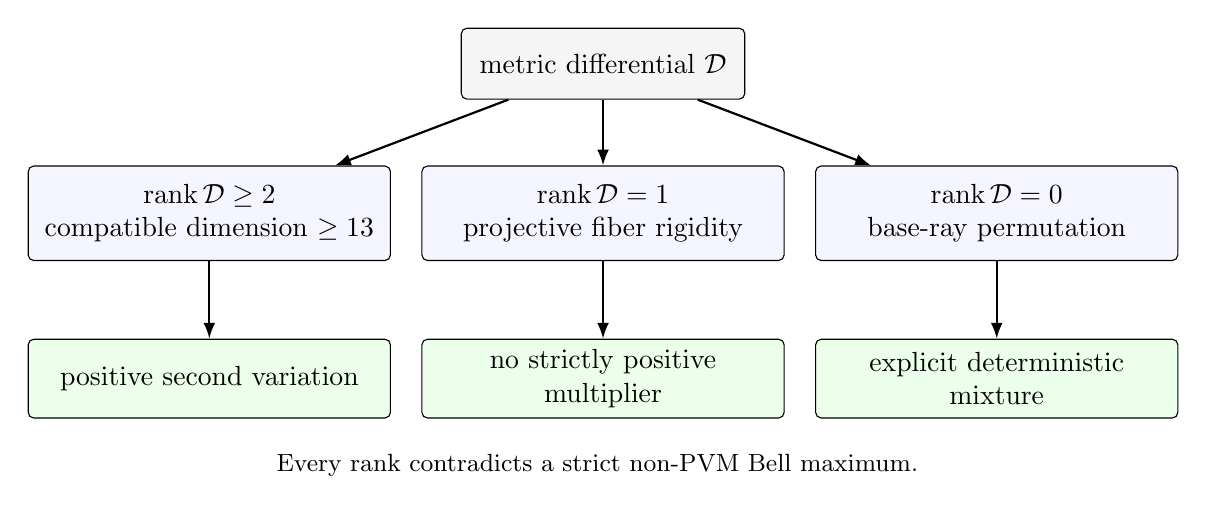
\begin{tikzpicture}[
  root/.style={draw,rounded corners=2pt,fill=gray!8,minimum width=3.6cm,
    minimum height=9mm,align=center},
  case/.style={draw,rounded corners=2pt,fill=blue!4,minimum width=4.6cm,
    minimum height=1.2cm,align=center},
  end/.style={draw,rounded corners=2pt,fill=green!8,minimum width=4.6cm,
    minimum height=1.0cm,align=center},
  arr/.style={-{Latex[length=2mm]},thick}
]
\node[root] (d) at (0,1.8) {metric differential \(\mathcal D\)};
\node[case] (r2) at (-5,-0.1) {
  \(\operatorname{rank}\mathcal D\ge2\)\\
  compatible dimension \(\ge13\)
};
\node[case] (r1) at (0,-0.1) {
  \(\operatorname{rank}\mathcal D=1\)\\
  projective fiber rigidity
};
\node[case] (r0) at (5,-0.1) {
  \(\operatorname{rank}\mathcal D=0\)\\
  base-ray permutation
};
\node[end] (e2) at (-5,-2.2) {positive second variation};
\node[end] (e1) at (0,-2.2) {no strictly positive\\multiplier};
\node[end] (e0) at (5,-2.2) {explicit deterministic\\mixture};
\draw[arr] (d) -- (r2);
\draw[arr] (d) -- (r1);
\draw[arr] (d) -- (r0);
\draw[arr] (r2) -- (e2);
\draw[arr] (r1) -- (e1);
\draw[arr] (r0) -- (e0);
\node[align=center,font=\small] at (0,-3.3) {
  Every rank contradicts a strict non-PVM Bell maximum.
};
\end{tikzpicture}
}
\caption{The exhaustive rank trichotomy for the metric differential.}
\label{fig:trichotomy}
\end{figure}

\subsection{Rank at least two}

If \(\rank\cD\ge2\), then \(k\le3\) and
\[
\dim\mathcal H_K=16-k\ge13.
\]
A subspace on which a form of inertia \((4,12)\) is nonpositive has dimension
at most \(12\): projection to its twelve negative coordinates is injective.
Therefore \(\mathcal H_K\) contains \(W\) with \(q(W)>0\). Normalize it using
\cref{prop:second-form} and integrate it using
\cref{thm:physical-completeness}. The resulting physical curve has positive
Bell second derivative, contradicting local maximality.

\subsection{Rank one}

The coefficient form of the metric differential is the quadratic map
\[
\Phi(y)=
\bigl(y_2(y_0+y_3),\,y_3(y_0+y_2),\,
y_2(y_1+y_3),\,y_3(y_1+y_2)\bigr)^T.
\]

\begin{proposition}[Projective fiber theorem]
\label{prop:fiber}
On the strict \(g\)-null quadric, the base locus of \(\Phi\) is exactly the
five coefficient rays \([r_1],\ldots,[r_5]\). Away from the base locus,
\(\Phi\) is projectively injective, including on the exceptional divisors
\[
y_2=0,\quad y_3=0,\quad y_0=y_1,\quad y_2=y_3.
\]
\end{proposition}

\begin{proof}
The generic rational inverse and the exact exceptional-divisor calculations
are given in \cref{app:fibers}. Each resultant and factorization is reproduced
by the exact verifier. The strict metric inequalities exclude extra null
roots without excluding any genuine residual point.
\end{proof}

If \(\rank\cD=1\), all nonzero \(\Phi(y_j)\) are projectively equal.
The five \(y_j=QPr_j\) are distinct rays because \(QP\) is invertible.
\Cref{prop:fiber} therefore permits at most one nonzero row of \(\cD\).
Consequently
\[
\ker\cD^T=\{\mu:\mu_{j_0}=0\}
\]
for some \(j_0\), which contains no strictly positive vector. This
contradicts \(\lambda_j>0\).

\subsection{Rank zero}

If \(\rank\cD=0\), every \(y_j\) belongs to the five-ray base locus.
Invertibility gives
\[
y_j=t_jr_{\pi(j)},\qquad t_j>0,
\]
for a permutation \(\pi\). The unique circuit forces \(\pi\) to preserve the
binary and ternary partitions and all \(t_j\) to be equal. Normalization fixes
the common scale, so after relabeling
\[
QP=\id,\qquad P=g.
\]

\begin{proposition}[Rank-zero deterministic simulation]
\label{prop:rank-zero}
Every rank-zero probability table \(p_{ij}=r_i^Tgr_j\) is a convex
combination of deterministic local behaviors, and hence belongs to
\(\Qbar^{\PVM}_2\).
\end{proposition}

\begin{proof}
Let \(c_{ij}\) be the ternary--ternary block, with \(c_{ii}=0\), and let
\(a_i,b_i\) be the two binary--ternary rows. They obey
\[
\sum_{j\ne i}c_{ij}=a_i+b_i,\qquad
\sum_i a_i=\sum_i b_i=\frac12.
\]
\Cref{app:transport} constructs a matrix \(q_{ij}\) satisfying
\[
0\le q_{ij}\le c_{ij},\qquad
\sum_jq_{ij}=b_i,\qquad
\sum_iq_{ij}=a_j.
\]
For each ordered ternary pair \((i,j)\), assign weight \(q_{ij}\) to the
deterministic binary outputs \((1,2)\), and weight \(c_{ij}-q_{ij}\) to
\((2,1)\), while fixing ternary outputs to \((i,j)\). Summing these branches
reproduces the ternary block, both mixed blocks, and the binary block
simultaneously. Identity and zero projectors implement every deterministic
branch.
\end{proof}

\subsection{Equality}

\begin{theorem}[Universal two-input equality]
\label{thm:two-input-equality}
For every finite input-dependent output architecture
\((A_0,A_1;B_0,B_1)\),
\[
\boxed{
\Qbar^{\POVM}_2(\mathbf A,\mathbf B)
=
\Qbar^{\PVM}_2(\mathbf A,\mathbf B).
}
\]
\end{theorem}

\begin{proof}
The PVM-to-POVM inclusion is immediate. Suppose the reverse inclusion failed.
The nearest-point argument in \cref{lem:nearest} would give a Bell functional
whose global POVM maximum strictly exceeds its PVM maximum. Choose an extreme
point of its exposed maximizing face. By
\cref{thm:residual-reduction}, a maximizing component lies in the genuine
residual architecture. Every local measurement is therefore globally optimal
with the other variables fixed, so \cref{prop:positive-multipliers} applies.

The metric differential has rank \(0,1,2,3,\) or \(4\). Rank at least two has
an uphill physical direction; rank one cannot carry the required positive
multiplier; rank zero is PVM-simulable by \cref{prop:rank-zero}. Every case
contradicts a strict value above the PVM support function.
\end{proof}

\begin{corollary}[Minimum input architecture]
\label{cor:minimality}
Up to exchanging the parties, \(3\times2\) is the minimum input architecture
for a strict fixed-qubit POVM-over-PVM Bell separation.
\end{corollary}

\begin{proof}
With one input on either party every nonsignaling behavior is local, hence a
deterministic PVM behavior maximizes every Bell functional. Two inputs on both
parties are excluded by \cref{thm:two-input-equality}.
\Cref{thm:separation} supplies an exact \(3\times2\) separation.
\end{proof}

\section{Operational consequences and limitations}

For every Bell functional with two inputs per party, optimizing over
fixed-qubit PVMs already
provides the fixed-qubit POVM bound. Thus a value above that bound excludes
all local-qubit realizations, not merely projective ones.

Likewise, no qubit behavior with two inputs per party can certify that a
nonprojective local
measurement was indispensable: after shared-randomness convexification, a
PVM realization always exists. This does not identify the state or
measurements in a particular laboratory realization, and it does not assert
raw-set equality without shared randomness.

We do not claim the exact global POVM or PVM optimum of
\eqref{eq:bell-functional}. We also do not infer a private-randomness entropy
bound: such a statement requires an adversarial extension of the convex
decomposition, not only equality of observed behavior sets.

\section{Discussion}

The threshold result is special to local dimension two. Natural open
questions include minimum-input laws in dimension three and higher,
multipartite scenarios, equality without convexification, constructive
simulation algorithms for generic two-input behaviors, instruments and
sequential measurements, and experimentally robust exact \(3\times2\)
witnesses. Determining the exact two-qubit POVM and PVM optima of
\eqref{eq:bell-functional} is also open but unnecessary for the separation.

The proof illustrates a distinction between operator-level and behavioral
generality. Ternary qubit POVMs are genuine generalized measurements, yet two
inputs do not provide enough Bell structure to make them indispensable after
the state and shared-randomness decomposition may change. A third input can
lock the state and steering geometry while reserving another measurement for
a discrimination advantage.

\section*{Data, code, and verification}

The accompanying repository contains exact Bell coefficients and strategies,
the separation verifier, the exceptional-fiber identities, the closure
verifier, and an independent rank-zero simulator. One offline command runs
all exact checks. The code verifies finite algebraic identities and explicit
constructions; the convexity, extremality, physical-reconstruction, and
dimension arguments remain human proofs in this manuscript.

\section*{AI-assisted research and verification}

Generative-AI systems were used extensively during mathematical exploration,
symbolic derivation, adversarial proof analysis, software development, and
preparation of the manuscript in July 2026. The final arguments and
computational artifacts were assembled under the responsibility of the human
author, who takes full responsibility for all claims, proofs, citations, and
released materials. Generative-AI systems are not listed as authors. The
included exact verifiers were implemented separately from several discovery
calculations, but no claim of independent expert human verification is made.

\section*{Competing interests and funding}

The author declares no competing interests. This research received no
external funding.

\appendix
\section[Exact algebra for the 3-by-2 separation]
{Exact algebra for the \(3\times2\) separation}
\label{app:separation-algebra}

We record the identities that make the projective bound independent of
numerical optimization. For a pair involving auxiliary label \(2\), let
\[
A=\frac35D \Pi(\bm n)D,\qquad
B=\frac45D \Pi(\bm m)D,
\]
where \(x=n_z\), \(y=m_z\), \(r=\bm n\cdot\bm m\), and
\[
D=\operatorname{diag}\!\left(
\sqrt{\frac{1+\eta}{2}},\sqrt{\frac{1-\eta}{2}}\right).
\]
Direct expansion, using \(\|\bm n\|=\|\bm m\|=1\), gives
\[
\det(A-B)=-\frac3{50}(1-\eta^2)(1-r)\le0.
\]
Thus \(A-B\) has eigenvalues of opposite signs, including a possible zero
boundary eigenvalue, and the optimized complementary-projector score is
\[
F_\eta=\frac{\Tr A+\Tr B+\|A-B\|_1}{2}.
\]
Its discriminant yields
\[
20F_\eta=
7+\eta(3x+4y)+
\sqrt{[-1+\eta(3x-4y)]^2+24(1-\eta^2)(1-r)}.
\]

At \(\eta=0\),
\[
F_0(r)=\frac7{20}+\frac1{20}\sqrt{25-24r}.
\]
Set
\[
q=\sqrt{25-24r}\ge1,\qquad H=8-3x-4y\ge1.
\]
To prove \(F_\eta\le F_0(r)+2\eta/5\), it is enough to prove
\[
\sqrt{[-1+\eta(3x-4y)]^2+24(1-\eta^2)(1-r)}
\le q+\eta H.
\]
The right side is at least one, so squaring is valid. Using
\(q^2=25-24r\), the squared difference is exactly
\[
\begin{aligned}
2\eta\{&
\eta[8(1-y)(4-3x)+12(1-r)]\\
&+(q-1)(8-3x-4y)+8(1-y)\}.
\end{aligned}
\]
Every factor is nonnegative on
\[
0\le\eta\le1,\qquad -1\le x,y,r\le1.
\]
No omitted compatibility condition among \(x,y,r\) can invalidate the
estimate because it holds on the larger box.

For \(u=|\bm b_0\cdot\bm b_1|\), both relevant pairs satisfy \(r\ge-u\).
Moreover,
\[
(5+8u)^2-(25+24u)=8u(7+8u)\ge0,
\]
so
\[
F_0(r)\le\frac7{20}+\frac1{20}\sqrt{25+24u}
\le\frac35+\frac{2u}{5}.
\]

For completeness, the scalar inequalities in the CHSH-deficit estimate have
nonnegative squared differences
\[
\left(1-\frac{u^2}{2}\right)^2-(1-u^2)=\frac{u^4}{4},
\]
\[
\left(2-\frac{u^2}{4}\right)^2-(4-u^2)=\frac{u^4}{16}.
\]
Their right sides are nonnegative on \(0\le u\le1\), so no sign reversal is
introduced by squaring.

\section{The strengthened algebraic strategy}
\label{app:strengthened}

Put
\[
q=\sqrt{7813},\qquad \eta=\frac1q,\qquad
s=\sqrt{1-\eta^2}=\frac{6\sqrt{217}}q.
\]
Use
\[
|\psi_\eta\rangle=
\sqrt{\frac{1+\eta}{2}}|00\rangle+
\sqrt{\frac{1-\eta}{2}}|11\rangle,
\]
Bob observables \(B_0=X,B_1=Z\), and Alice observables
\[
A_0=\frac{6\sqrt{217}\,X+qZ}{125},\qquad
A_1=\frac{6\sqrt{217}\,X-qZ}{125}.
\]
They square to the identity because
\[
36\cdot217+7813=125^2.
\]
The CHSH value is \(S=250/q\).

Set
\[
k=\frac35\sqrt{\frac{q-1}{q+1}}
\]
and
\[
M_0=\frac12\begin{pmatrix}k^2&k\\k&1\end{pmatrix},\qquad
M_1=\frac12\begin{pmatrix}k^2&-k\\-k&1\end{pmatrix},\qquad
M_2=\begin{pmatrix}1-k^2&0\\0&0\end{pmatrix}.
\]
These are positive rank-one effects and sum to the identity. The diagonal
dual operator
\[
\Gamma=
\operatorname{diag}\!\left(
\frac25(1+\eta),\frac6{25}(1-\eta)\right)
\]
dominates all three weighted steered score operators and annihilates the
corresponding effect ranges. Hence
\[
T=\Tr\Gamma=\frac{16+4\eta}{25},
\qquad
10S+T=\frac{16+8q}{25}.
\]

Within this one-parameter family,
\[
f(\eta)=20\sqrt{2-\eta^2}+\frac{16+4\eta}{25}
\]
has
\[
f'(\eta)=-\frac{20\eta}{\sqrt{2-\eta^2}}+\frac4{25},\qquad
f''(\eta)=-\frac{40}{(2-\eta^2)^{3/2}}<0.
\]
Its unique critical point is \(\eta=1/\sqrt{7813}\). This is not a global
POVM optimality claim.

Finally,
\[
(6+80\sqrt{7813})^2-2\cdot5003^2
=-56782+960\sqrt{7813},
\]
and
\[
960^2\cdot7813-56782^2=3\,976\,265\,276>0.
\]
Both sides being compared are positive, these two exact square comparisons
prove \(L_1>U\).

\section{Degenerate cases in the one-binary-party theorem}
\label{app:binary-degeneracies}

If \(B_0,B_1\) are nondegenerate and have linearly independent Bloch axes,
\(\Phi_B\) maps the positive cone onto a three-dimensional Lorentz cone.
An extreme ray of the image lies on the boundary ellipse. Its minimum-norm
Bloch lift in the plane of the two axes has norm one; a perpendicular
component would exceed the Bloch ball. Thus the positive lift in
\(\operatorname{span}_{\R}\{\id,B_0,B_1\}\) is unique and rank one.

If the Bloch axes are parallel or antiparallel, the image is the cone over an
interval and has two extreme rays. Every positive relation reduces to
one-versus-one cancellations or a two-versus-two relation with repeated
zero-padded outcomes. The same purification construction applies.

If one observable is scalar and the other nondegenerate, the image is again
two-dimensional; the scalar input is deterministic and does not add a
coordinate. If both are scalar, Bob is deterministic on both inputs and the
behavior is local. A rank-deficient circuit sum \(\Omega\) forces all lifted
rays to be collinear and is realized by a product purification. Zero effects
receive zero projectors. These cases also show that circuit weights remain
nonnegative and sum to one at the boundary.

\section{Extremal qubit POVMs and the rank-square bound}
\label{app:extremal-povm}

Let \(M_a\) be the nonzero effects of a POVM. For each \(a\), let
\(\mathcal V_a\) be the real vector space of Hermitian operators supported on
\(\operatorname{ran}M_a\). It has dimension \(\rank(M_a)^2\).
Consider the summation map
\[
\bigoplus_a\mathcal V_a\longrightarrow\Herm(2),\qquad
(H_a)_a\longmapsto\sum_aH_a.
\]
If it has a nonzero kernel, then for sufficiently small \(\eps>0\),
\(M_a\pm\eps H_a\ge0\), and the two perturbed tuples are distinct POVMs whose
average is \(M\). Extremality therefore requires injectivity, giving
\[
\sum_a\rank(M_a)^2\le\dim_{\R}\Herm(2)=4.
\]
This necessary condition is all that is used in
\cref{thm:residual-reduction}. Together with linear independence in a
three-dimensional span, it leaves exactly three rank-one effects.

\section{Finite-dimensional POVM duality}
\label{app:duality}

Let
\[
V=\max_{\substack{N_j\ge0\\\sum_jN_j=\id}}
\sum_j\Tr(K_jN_j).
\]
Weak duality says that every \(\Gamma\ge K_j\) obeys
\[
\sum_j\Tr(K_jN_j)\le\Tr\Gamma.
\]
For the reverse direction, consider the closed cone
\[
\mathcal C=
\left\{\left(\sum_jX_j,\sum_j\Tr(K_jX_j)-t\right):
X_j\ge0,\ t\ge0\right\}
\subset\Herm(2)\times\R.
\]
Closedness follows because convergence of \(\sum_jX_j\) bounds every
\(0\le X_j\le\sum_kX_k\).

The point \((\id,V+\eps)\) is outside \(\mathcal C\). Nearest-point
separation provides a nonzero functional
\[
\ell(A,s)=\Tr(\Gamma_\eps A)+\gamma s
\]
nonnegative on \(\mathcal C\) and negative at that point. Since
\((0,-t)\in\mathcal C\), \(\gamma\le0\). If \(\gamma=0\), positivity on all
\((X,\Tr(K_jX))\) would give \(\Gamma_\eps\ge0\), contradicting
\(\Tr\Gamma_\eps<0\). Normalize \(\gamma=-1\). Taking one nonzero \(X_j=X\)
gives \(\Gamma_\eps\ge K_j\), while separation and weak duality give
\[
V\le\Tr\Gamma_\eps<V+\eps.
\]
A bounded convergent subsequence as \(\eps\downarrow0\) yields dual
attainment with \(\Tr\Gamma=V\).

At a primal optimum,
\[
0=\Tr\Gamma-\sum_j\Tr(K_jN_j)
=\sum_j\Tr[(\Gamma-K_j)N_j].
\]
Each term is nonnegative, hence zero. For \(A,B\ge0\),
\(\Tr(AB)=0\) implies \(A^{1/2}BA^{1/2}=0\), and therefore \(AB=0\).
This proves complementary slackness.

\section{Square completion for the incidence Hessian}
\label{app:square-completion}

Let \(x_j=Pr_j\), \(Q=g^{-1}\), and vary
\[
P(t)=P+t\delta P,\qquad g(t)=g+tH
\]
to first order. The inverse expansion is
\[
(g+tH)^{-1}
=Q-tQHQ+t^2QHQHQ+O(t^3).
\]
Substitution in \(F_j=(P r_j)^TQ(P r_j)\) gives
\[
\begin{aligned}
\frac12D^2F_j
={}&(\delta P r_j)^TQ(\delta P r_j)
-2(\delta P r_j)^TQHQ(Pr_j)\\
&+(Pr_j)^TQHQHQ(Pr_j).
\end{aligned}
\]
Writing
\[
\delta P=PW+HQ P
\]
turns the right side into
\[
(PWr_j)^TQ(PWr_j).
\]
Therefore
\[
\sum_j\lambda_jD^2F_j
=2\sum_j\lambda_jr_j^TW^TP^TQPW r_j
=2\Tr(SW\Lambda W^T).
\]
This expansion also fixes the sign convention used at a Bell maximum.

\section{Projective fibers of the quadratic null-ray map}
\label{app:fibers}

Let
\[
\mathcal N_g=\{[x]\in\mathbb{RP}^3:x^Tgx=0\}
\]
for a strict metric \eqref{eq:metric}, and write
\(\Phi(x)=(A,B,C,D)\).

\subsection{Base locus and generic inverse}

If \(x_2=x_3=0\), nullness gives \(x_0x_1=0\), hence \(r_1,r_2\).
If exactly one of \(x_2,x_3\) vanishes, the remaining equations give
\(r_3\) or \(r_4\). If \(x_2x_3\ne0\), all four components of \(\Phi\)
vanish only when
\[
x_0=x_1=-x_2=-x_3,
\]
the ray \(r_5\). Thus the base locus consists exactly of the five coefficient
rays.

The identities
\[
\begin{aligned}
A-B&=x_0(x_2-x_3),&
C-D&=x_1(x_2-x_3),\\
A-C&=x_2(x_0-x_1),&
B-D&=x_3(x_0-x_1),\\
AD-BC&=x_2x_3(x_0-x_1)(x_2-x_3)
\end{aligned}
\]
give
\[
\begin{pmatrix}
(A-B)(A-C)(B-D)\\
(C-D)(A-C)(B-D)\\
(AD-BC)(A-C)\\
(AD-BC)(B-D)
\end{pmatrix}
=\omega(x)x,
\]
where
\[
\omega(x)=x_2x_3(x_2-x_3)(x_0-x_1)^2.
\]
Hence \([x]\) is recovered from \([\Phi(x)]\) whenever \(\omega(x)\ne0\).

\subsection[Exceptional divisor x2=0]{Exceptional divisor \(x_2=0\)}

The target is \([0:B:0:D]\). On the direct branch, scale \(z_3=1\) and
write \((z_0,z_1)=t(B,D)\). Nullness is
\[
t^2BD+2t(bB+dD)=0.
\]
The root \(t=0\) is \(r_4\), leaving at most one nonbase root. On the cross
branch \(z_2\ne0\), target zeros force \(z_0=z_1=-z_3\) and a nonzero target
requires \(B=D\). With \(z_3=1,z_2=t\),
\[
z^Tgz=(1-2(b+d))(1-t).
\]
Strictness \(b+d<1/2\) gives only \(t=1\), the base ray \(-r_5\).

\subsection[Exceptional divisor x3=0]{Exceptional divisor \(x_3=0\)}

The symmetric direct equation is
\[
t^2AC+2t(aA+cC)=0,
\]
and the cross equation is
\[
(1-2(a+c))(1-t)=0.
\]
Again there is at most one nonbase preimage.

\subsection[Exceptional divisor x0=x1]{Exceptional divisor \(x_0=x_1\)}

If \(x_0=x_1=0\), nullness reduces to \(2e x_2x_3=0\). Since \(e>0\),
the point is \(r_3\) or \(r_4\), hence in the base locus. A nonbase point may
therefore be scaled to \(x_0=x_1=1\). Put \(p=x_2,q=x_3\). The null and
target-ratio equations are
\[
N=1+2(a+c)p+2(b+d)q+2epq=0,
\]
\[
R=Bp(1+q)-Aq(1+p)=0.
\]
Their exact resultant in \(p\) is
\[
\operatorname{Res}_p(N,R)
=-(q+1)\left[
B+q\bigl(A(2a+2c-1)+2B(b+d)\bigr)
\right].
\]
At \(q=-1\), strictness gives \(p=-1\), the base ray. The second factor is
not identically zero: if \(B\ne0\) its constant term is nonzero; if \(B=0\),
then \(A\ne0\) and \(2(a+c)-1\ne0\). Once \(q\) is fixed, \(N\) determines
at most one \(p\). The only apparent failure would require
\[
2(a+c)(b+d)=a+b+c+d-\tfrac12,
\]
equivalent to
\[
(2(a+c)-1)(2(b+d)-1)=0,
\]
which strictness excludes.

\subsection[Exceptional divisor x2=x3]{Exceptional divisor \(x_2=x_3\)}

If \(x_2=x_3=0\), nullness gives \(x_0x_1=0\), hence the base rays
\(r_1,r_2\). For a nonbase point scale \(x_2=x_3=1\) and put
\(p=x_0,q=x_1\). The equations are
\[
N=pq+2(a+b)p+2(c+d)q+2e=0,
\]
\[
R=C(p+1)-A(q+1)=0.
\]
The exact resultant is
\[
\operatorname{Res}_p(N,R)
=-(q+1)\left[
Aq+2A(a+b)+2C(c+d)-C
\right].
\]
At \(q=-1\), strictness gives \(p=-1\), the base ray. Strictness also excludes
an identically vanishing second factor or an undetermined null equation.

For a possible cross-branch preimage with \(z_2\ne z_3\), equal target
coordinates give \(z_0=z_1=0\); strict \(e>0\) and nullness then force
\(z_2z_3=0\), again a base ray. These cases exhaust \(\omega=0\), proving
projective injectivity away from the base locus.

\section{Bounded transportation and the rank-zero simulation}
\label{app:transport}

For three ternary labels, let \(c_{ij}=c_{ji}\ge0\), \(c_{ii}=0\), and assume
\[
\sum_{j\ne i}c_{ij}=a_i+b_i,\qquad
\sum_i a_i=\sum_i b_i=\frac12.
\]
Seek \(q_{ij}\) with row sums \(b_i\), column sums \(a_j\), and
\(0\le q_{ij}\le c_{ij}\). Put
\[
q_{ij}=\frac{c_{ij}}2+f_{ij},\qquad f_{ij}=-f_{ji},
\]
\[
d_i=\frac{b_i-a_i}{2},\qquad d_1+d_2+d_3=0.
\]
Set
\[
f_{12}=t,\qquad f_{13}=d_1-t,\qquad f_{23}=d_2+t.
\]
The row and column equations are automatic. Capacity is equivalent to
\[
t\in I_{12}\cap I_{13}\cap I_{23},
\]
where
\[
\begin{aligned}
I_{12}&=[-c_{12}/2,c_{12}/2],\\
I_{13}&=[d_1-c_{13}/2,d_1+c_{13}/2],\\
I_{23}&=[-d_2-c_{23}/2,-d_2+c_{23}/2].
\end{aligned}
\]
The inequalities
\[
|d_i|\le\frac{a_i+b_i}{2}
=\frac{c_{ij}+c_{ik}}2
\]
show that every pair of intervals intersects, including zero-capacity
endpoints. Three closed intervals on the real line with pairwise
intersections have a common point: the largest left endpoint does not exceed
the smallest right endpoint. Any common \(t\) gives the required bounded
transportation matrix.

The deterministic branch construction in
\cref{prop:rank-zero} then reproduces all four input blocks simultaneously.
The supplied rational simulator independently checks the construction on an
interior symmetric instance; generality follows from the interval proof, not
from that one executable example.

\section{Verification boundary}
\label{app:verification}

The exact verifier checks:
\begin{enumerate}[leftmargin=*]
\item dense and sparse Bell coefficients and both explicit strategies;
\item POVM normalization, rank-one factorizations, exact Bell values, and
  discrimination dual certificates;
\item the determinant, discriminant, robust-comparison, deficit, and
  complete-square identities in the projective bound;
\item the Lorentz metric identities, quadratic map, generic inverse, all
  exceptional resultants and factorizations;
\item an exact pure-state conformal-Lorentz instance and the weighted Hessian
  square completion;
\item independence witnesses for the five incidence constraints;
\item bounded-flow identities and an independent rank-zero simulation.
\end{enumerate}

The scripts do not replace the human arguments establishing compactness,
extremal reduction, cone circuits, physical completeness, multiplier signs,
dimension bounds, or exhaustion of cases. Some symbolic checks are exact
regression instances rather than formal proofs of general matrix identities;
the corresponding general identities are derived above.


\begingroup
\small
\setlength{\bibsep}{2pt}
\bibliographystyle{unsrtnat}
\bibliography{references}
\endgroup

\end{document}
